Primero vamos a analizar el peso total del resultado devuelto por nuestro algoritmo de GRASP frente a distintas soluciones iniciales. Vamos a utilizar como soluciones iniciales a nuestro algoritmo goloso, y el resultado de recorrer el algoritmo de Dijkstra sobre la función de peso $\omega_1$.

En la figura \ref{fig:grasp-soluciones-iniciales} incluimos un gráfico tipo \emph{scatter} con los puntos que tienen como coordenadas $x$ e $y$ los valores de $W_2$ obtenidos utilizando los diferentes tipos de solución inicial, respectivamente, sobre instancias aleatorias de múltiples $n$.

\begin{figure}[H]
  \begin{center}
    \begin{minipage}{0.7\linewidth}
      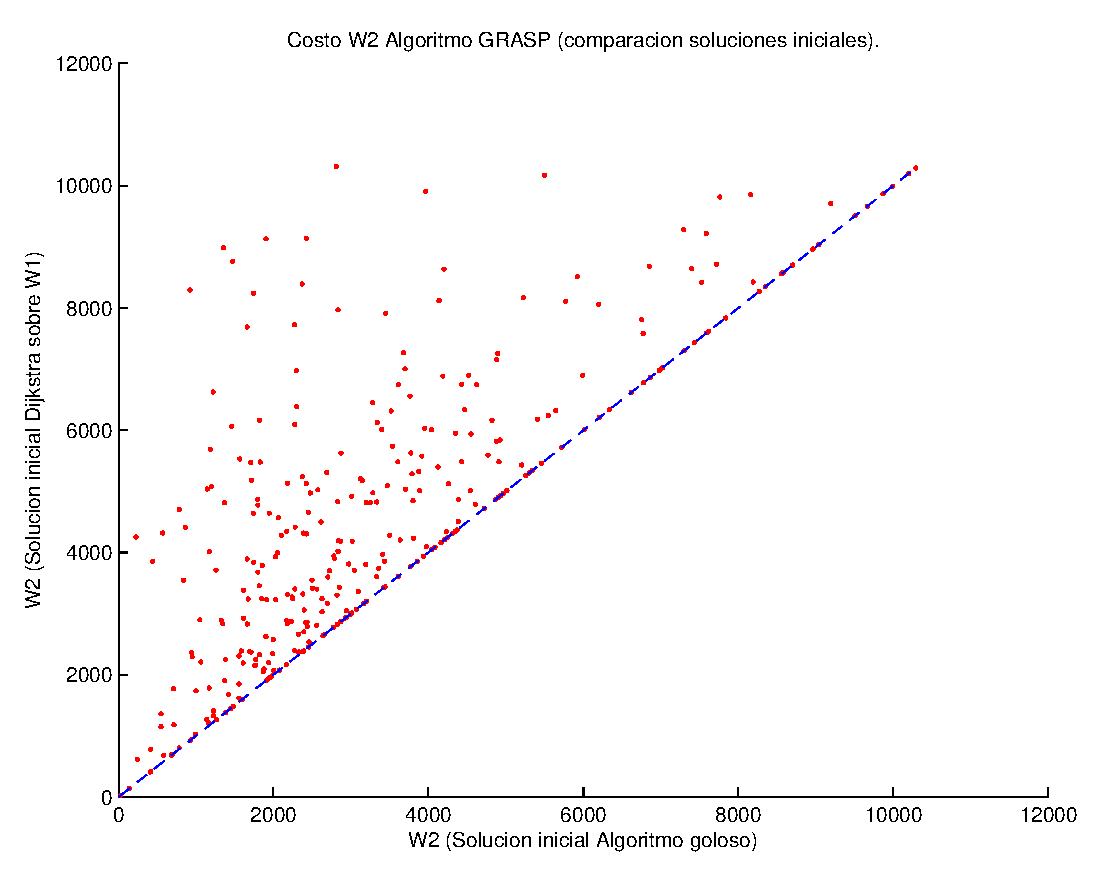
\includegraphics[width=\linewidth]{graficos/grasp_comparacion_soluciones_iniciales.eps}
      \caption{Comparación de los valores de $W_2$ obtenidos para las distintas soluciones iniciales}\label{fig:grasp-soluciones-iniciales}
    \end{minipage}
  \end{center}
\end{figure}

Como podemos observar en el gráfico, frente a casos al azar, utilizar como solución inicial nuestro algoritmo goloso es mejor o igual que utilizar Dijkstra sobre $\omega_1$. Para facilitar la lectura, imprimimos una línea azul que representa a la función identidad.

Dado que el análisis previo ignora el efecto del tamaño del grafo en la relación entre ambos valores de $W_2$, incluimos el siguiente gráfico en la figura \ref{fig:grasp-soluciones-iniciales-tiempo} mostrando la proporción entre los mismos, en función de $n$:

\begin{figure}[H]
  \begin{center}
    \begin{minipage}{0.7\linewidth}
      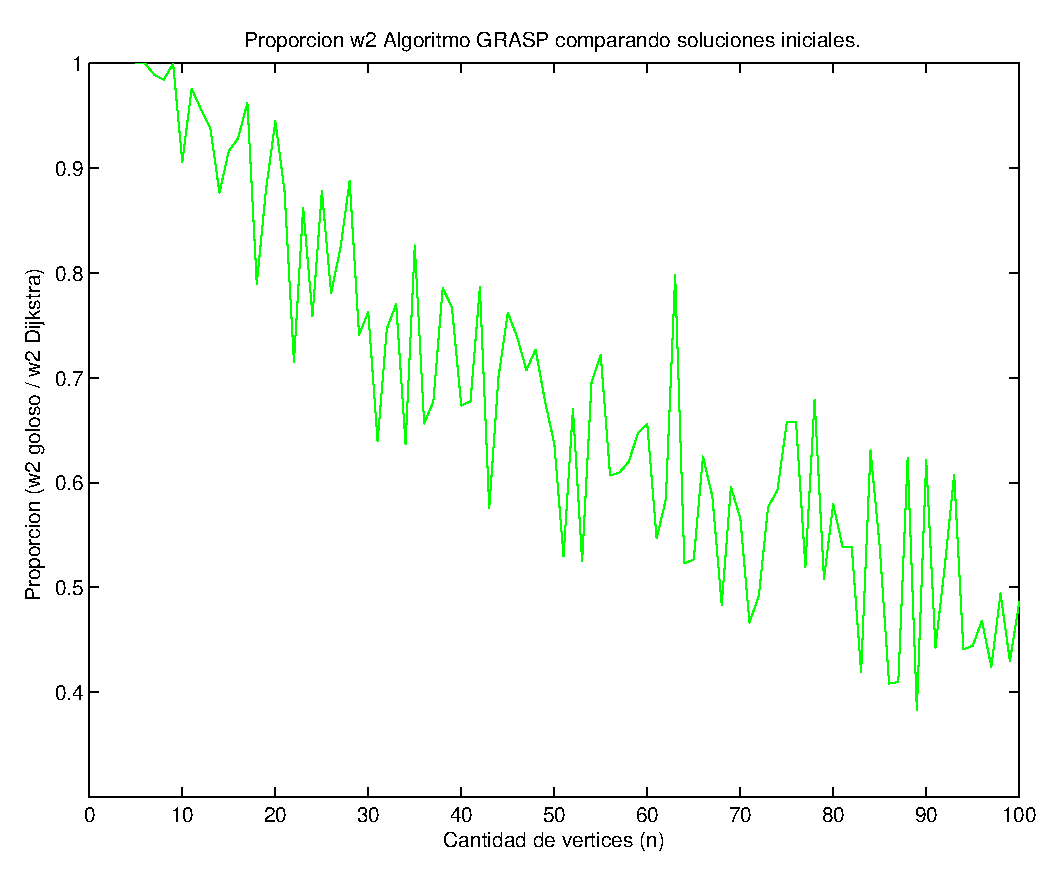
\includegraphics[width=\linewidth]{graficos/grasp_comparacion_soluciones_iniciales_tiempo.eps}
      \caption{Proporción de los valores de $W_2$ obtenidos para las distintas soluciones iniciales, en función de $n$.}\label{fig:grasp-soluciones-iniciales-tiempo}
    \end{minipage}
  \end{center}
\end{figure}


Como ya habíamos visto antes, usar como solución inicial nuestro algoritmo goloso siempre da mejores soluciones que usando Dijkstra, por eso todos los valores son inferiores a 1 (goloso $<$ Dijkstra). Algo interesante que deducimos de este ultimo gráfico, es que a medida que el $n$ crece, el beneficio de usar el algoritmo goloso como solución inicial es cada vez mejor en comparación con usar Dijkstra.

Creemos que esto ocurre ya que las soluciones que encuentra Dijkstra, aunque tiene una componente aleatoria, van a tener un $w_1$ bajo pero posiblemente un $w_2$ alto. En cambio, el goloso busca soluciones más intermedias, no solo usando $w_1$. Creemos que al aumentar el $n$ la distancia entre estas soluciones borde de Dijkstra y las soluciones intermedias del goloso crece, generando el comportamiento observado en el gráfico.